\documentclass[10pt,letterpaper]{report}

\usepackage{iftex}
\ifPDFTeX
    \usepackage[T1]{fontenc}
    \usepackage[utf8]{inputenc}
    \usepackage{helvet}
    \renewcommand{\familydefault}{\sfdefault}
\else
    \usepackage{fontspec}
    \setmainfont{Arial}
\fi
\usepackage[spanish]{babel}
\usepackage[top=20mm,bottom=20mm,left=25mm,right=25mm]{geometry}
\setlength{\parskip}{5pt}
\usepackage{parskip}
\usepackage{titlesec}
\usepackage{xurl}
\usepackage{hyperref}
\hypersetup{colorlinks=true, linkcolor=black, urlcolor=blue, citecolor=black}
\usepackage{graphicx}
\usepackage{grffile}   % manejo de rutas con espacios
\usepackage{enumitem}
\usepackage{booktabs}
\usepackage{caption}
\usepackage{tocloft}
\usepackage{indentfirst}
\usepackage{longtable}
\usepackage{array}
\usepackage{tabularx}
\usepackage{amsmath}
\usepackage{amssymb}
\usepackage{pifont}    % \checkmark y \xmark

\counterwithout{figure}{chapter}
\counterwithout{table}{chapter}

\newcommand{\citeref}[2]{\hyperlink{ref:#1}{(#2)}}
\newcommand{\fechaentrega}{11 de junio de 2026}
\newcommand{\cmark}{\ding{51}}   % marca de aprobado

% ---------------------------------------------------------------------------
% Rutas de búsqueda de imágenes
% Copiar las imágenes de Casos de Prueba al directorio del .tex o ajustar la
% ruta según la estructura local antes de compilar.
% ---------------------------------------------------------------------------
\graphicspath{{./}{../../Casos de Prueba/}}

% Formato de títulos
\titleformat{\chapter}[block]{\large\bfseries}{}{0em}{}
\titlespacing*{\chapter}{0pt}{12pt}{6pt}
\titleformat{\section}[block]{\normalsize\bfseries}{\thesection}{1em}{}
\titleformat{\subsection}[block]{\normalsize\bfseries}{\thesubsection}{1em}{}
\titleformat{\subsubsection}[block]{\normalsize\bfseries}{\thesubsubsection}{1em}{}

\setcounter{secnumdepth}{3}
\setcounter{tocdepth}{3}

\begin{document}

% ===========================================================================
% PORTADA
% ===========================================================================
\begin{titlepage}
\centering
\vspace*{1cm}

\includegraphics[width=4.2cm]{logo.png}\\[1.2cm]
{\large\textbf{Instituto Tecnológico y de Estudios Superiores de Monterrey}}\\[0.4cm]
{\normalsize Escuela de Ingeniería y Ciencias}\\[0.2cm]
{\normalsize Ingeniería en Ciencia de Datos y Matemáticas}\\[1.5cm]
{\large\textbf{Gestor de Identidades y Registro de Migrantes}}\\[1.5cm]
{\normalsize\textbf{Casa Monarca --- Ayuda Humanitaria al Migrante A.B.P}}\\[1.5cm]
{\normalsize\textbf{Profesores:}}\\[0.3cm]
{\normalsize Raúl Gómez Muñoz \quad Alberto Francisco Martínez Herrera}\\
{\normalsize Pedro Leonel Olaya Trejos \quad Daniel Otero Fadul}\\[1.5cm]
{\normalsize\textbf{Equipo 1 --- Grupo 602}}\\[0.3cm]
{\normalsize
Mariel Álvarez Salas \quad A01198828\\
Brisma Alvarez Valdez \quad A00839238\\
Emiliano Ruiz López \quad A01659693\\
Ana Sofia Nagao Alvarez \quad A01285034\\
Karen Aylen Estrada Ceferino \quad A00838403
}\\[1.5cm]
{Monterrey, Nuevo León. \fechaentrega}\\[1.4cm]
\end{titlepage}

% ===========================================================================
% ÍNDICES
% ===========================================================================
\tableofcontents
\newpage
\listoffigures
\newpage
\listoftables
\newpage

% ===========================================================================
% ABSTRACT
% ===========================================================================
\chapter*{Abstract}
\addcontentsline{toc}{chapter}{Abstract}

Casa Monarca es una organización de la sociedad civil que brinda apoyo humanitario, legal y psicosocial a personas migrantes en situación vulnerable. Debido a la naturaleza sensible de la información que gestiona (datos personales, documentos legales y expedientes de los migrantes) resulta fundamental contar con mecanismos de seguridad que protejan esos datos y garanticen su integridad. El reporte presenta el diseño e implementación de un sistema desarrollado en Django que integra dos módulos: un gestor de identidades para colaboradores (IAM) y un módulo de registro de migrantes. El módulo IAM permite el alta, baja, revocación y rastreo de colaboradores con certificados digitales X.509. El módulo de registro de migrantes permite crear expedientes con cifrado de campos sensibles mediante AES-256, firma digital ECDSA por registro, un flujo de aprobación escalonado por niveles de acceso (1--4) y la gestión de los derechos ARCO conforme a la Ley Federal de Protección de Datos Personales en Posesión de Particulares (LFPDPPP). Las herramientas de Django y MySQL fueron seleccionadas con base en la compatibilidad con el servidor con el que ya cuenta Casa Monarca. Los siguientes pasos incluyen el despliegue del sistema, la capacitación del personal y la migración a una autoridad certificadora de mayor madurez.

\newpage

% ===========================================================================
% 1. INTRODUCCIÓN
% ===========================================================================
\chapter{Introducción}

La migración de personas provenientes de países sudamericanos en México es motivada por su ubicación geográfica con respecto al país que generalmente es el objetivo final: Estados Unidos de América \citeref{zamora2018}{Zamora G., 2018}. Nuevo León recibió aproximadamente 268,647 migrantes en 2020 \citeref{inegi2020}{INEGI, 2020}. Con ese flujo de personas que salen de sus países buscando mejores condiciones, múltiples organizaciones buscan minimizar el impacto negativo de estas migraciones. Casa Monarca es una organización de la sociedad civil que brinda apoyo humanitario, legal y social a personas migrantes en situación vulnerable.

Una de las problemáticas enfrentadas por Casa Monarca es el tratamiento de los datos personales de los migrantes. Al manejar datos como los antes mencionados y debido a la naturaleza sensible de esta información, es fundamental garantizar que los datos se traten de forma segura, evitando su alteración, falsificación o uso indebido. Se busca fortalecer sus procesos digitales mediante herramientas criptográficas que permitan proteger la información que gestiona, ya que actualmente este tipo de organizaciones enfrentan retos relacionados con la autenticidad de documentos digitales, la protección de bases de datos y la validación de la identidad de quienes participan en sus procesos.

El presente reto propone el diseño e implementación de un sistema seguro para Casa Monarca que permita gestionar de forma confiable tanto las identidades de sus colaboradores como los expedientes de las personas migrantes que atiende. El sistema se dividió en dos etapas: gestión de identidades (IAM) y registro de migrantes. El módulo IAM permite realizar el alta, baja, revocación y rastreo de colaboradores con certificados digitales. El módulo de Registro de Migrantes permite crear expedientes bajo un flujo de aprobación por niveles, asegurando el cumplimiento de los derechos ARCO de los migrantes. La solución es compatible con los servidores que Casa Monarca ya utiliza, por lo que no representa ningún costo adicional.

% ===========================================================================
% 2. MARCO DE REFERENCIA
% ===========================================================================
\chapter{Marco de Referencia}

\section{Criptografía de clave pública}

La criptografía de clave pública (asimétrica) opera con un par de claves matemáticamente relacionadas: una clave pública, que puede distribuirse libremente, y una clave privada, que el propietario mantiene en secreto. Cualquier entidad puede cifrar un mensaje con la clave pública del destinatario, pero solo el poseedor de la clave privada puede descifrarlo. De forma simétrica, la firma digital se genera con la clave privada del firmante y puede verificarse mediante la clave pública correspondiente \citeref{katz2014}{Katz \& Lindell, 2014}.

La seguridad de los esquemas de clave pública descansa en la dificultad computacional de ciertos problemas matemáticos: la factorización de enteros grandes en RSA, o el logaritmo discreto en curvas elípticas (ECDLP) en los esquemas ECC. Este sistema emplea exclusivamente criptografía de curva elíptica para las operaciones de firma, por razones que se detallan en la sección siguiente.

\section{Criptografía de curva elíptica y ECDSA}

Una curva elíptica $E$ sobre un campo primo $\mathbb{F}_p$ se define mediante la ecuación de Weierstrass reducida:
\begin{equation}
    y^2 \equiv x^3 + ax + b \pmod{p},
    \label{eq:weierstrass}
\end{equation}
donde $a, b \in \mathbb{F}_p$ satisfacen la condición de no-singularidad $4a^3 + 27b^2 \not\equiv 0 \pmod{p}$. El conjunto de puntos $(x, y) \in \mathbb{F}_p^2$ que satisfacen la Ecuación~(\ref{eq:weierstrass}), junto con el punto en el infinito $\mathcal{O}$, forma un grupo abeliano $(E(\mathbb{F}_p), +)$ bajo la ley de adición de puntos \citeref{hankerson2004}{Hankerson et al., 2004}.

La seguridad de los esquemas ECC descansa en el ECDLP: dado un generador $G \in E(\mathbb{F}_p)$ de orden primo $n$ y un punto $Q = kG$ con $k \in \{1, \ldots, n{-}1\}$, calcular $k$ a partir de $Q$ y $G$ es computacionalmente infeasible para los parámetros de curva actuales. Los mejores algoritmos conocidos para resolver el ECDLP en curvas bien elegidas tienen complejidad $O(\sqrt{n})$, de modo que una curva de 256 bits proporciona aproximadamente $2^{128}$ operaciones de seguridad \citeref{johnson2001}{Johnson et al., 2001}.

El algoritmo ECDSA (\textit{Elliptic Curve Digital Signature Algorithm}) utiliza esta estructura para firmar y verificar mensajes. El proceso de firma de un mensaje $m$ con clave privada $d_A$ es:
\begin{enumerate}[leftmargin=*]
    \item Calcular $e = \text{SHA-256}(m)$.
    \item Seleccionar un nonce aleatorio $k \in \{1, \ldots, n{-}1\}$.
    \item Calcular el punto $R = kG$ y obtener $r = x_R \bmod n$.
    \item Calcular $s = k^{-1}(e + r \cdot d_A) \bmod n$.
    \item La firma es el par $(r, s)$.
\end{enumerate}
La verificación requiere únicamente la clave pública $Q_A = d_A G$ \citeref{johnson2001}{Johnson et al., 2001}. En el sistema se utiliza la curva de Koblitz \texttt{SECP256K1}, definida sobre $\mathbb{F}_p$ con $p = 2^{256} - 2^{32} - 977$ y coeficientes $a = 0$, $b = 7$. Esta curva ofrece 128 bits de seguridad con claves de 256 bits, frente a RSA que requiere 3{,}072 bits de módulo para el mismo nivel de seguridad, como se muestra en la Tabla~\ref{tab:keysizes} \citeref{nist2023}{NIST, 2023}.

\begin{table}[h!]
\centering
\caption{Tamaño de clave equivalente para 128 bits de seguridad (elaboración propia basada en \citeref{nist2023}{NIST, 2023}).}
\label{tab:keysizes}
\begin{tabular}{lcc}
\toprule
\textbf{Algoritmo} & \textbf{Tamaño de clave (bits)} & \textbf{Seguridad equivalente (bits)}\\
\midrule
RSA / DH     & 3{,}072 & 128 \\
ECDSA        &     256 & 128 \\
AES-256      &     256 & 256 \\
SHA-256      &     --- & 128 (resistencia a colisiones) \\
\bottomrule
\end{tabular}
\end{table}

\section{Cifrado simétrico AES-256}

El Estándar de Cifrado Avanzado (AES) fue adoptado por el NIST en 2001 como sustituto del algoritmo DES \citeref{nist2001aes}{NIST, 2001}. AES opera sobre bloques de 128 bits mediante una red de sustitución-permutación; la variante de 256 bits aplica 14 rondas, cada una formada por cuatro transformaciones: \textit{SubBytes} (sustitución no lineal mediante S-Box), \textit{ShiftRows} (permutación de filas), \textit{MixColumns} (mezcla lineal por columnas) y \textit{AddRoundKey} (combinación con la subclave de ronda derivada del calendario de claves).

Para el cifrado de campos sensibles en la base de datos (nombre, apellidos, fecha de nacimiento, teléfono y país de origen), el sistema emplea AES-256 a través de la biblioteca \textit{cryptography} de PyCa \citeref{pyca2024}{Python Cryptographic Authority, 2024}. El modo de operación empleado garantiza que registros con valores idénticos produzcan textos cifrados distintos, lo que evita ataques de análisis de frecuencia sobre la base de datos. Esto es especialmente relevante dado que los campos cifrados son datos personales de alta sensibilidad cuya re-identificación debe impedirse incluso en caso de acceso directo al almacenamiento.

\section{Función hash SHA-256 y cadenas de integridad}

SHA-256 (\textit{Secure Hash Algorithm, 256 bits}) pertenece a la familia SHA-2, estandarizada en NIST FIPS 180-4 \citeref{nist2015sha}{NIST, 2015}. La función acepta entradas de longitud arbitraria y produce un resumen de 256 bits (32 bytes). Sus propiedades criptográficas relevantes para este sistema son:
\begin{itemize}[leftmargin=*]
    \item \textbf{Resistencia a preimagen:} dado un resumen $h$, es computacionalmente infeasible encontrar $m$ tal que $\text{SHA-256}(m) = h$.
    \item \textbf{Resistencia a colisiones:} es computacionalmente infeasible encontrar $m_1 \neq m_2$ tal que $\text{SHA-256}(m_1) = \text{SHA-256}(m_2)$.
    \item \textbf{Efecto avalancha:} un cambio de un solo bit en la entrada altera aproximadamente la mitad de los bits del resumen.
\end{itemize}

El sistema utiliza SHA-256 en dos contextos distintos. Primero, como función de pre-hash antes de la firma ECDSA: el contenido de cada expediente se serializa y se calcula su resumen, que es el valor que se firma con ECDSA. Segundo, para implementar la cadena de auditoría criptográfica: cada firma del modelo \texttt{ActionSignature} incorpora en el campo \texttt{prev\_chain\_hash} el resumen SHA-256 de la firma anterior, formando una estructura encadenada en la que cualquier alteración retroactiva del historial es detectable \citeref{nakamoto2008}{Nakamoto, 2008}.

\section{Infraestructura de clave pública (PKI) y certificados X.509}

Una infraestructura de clave pública (PKI) define las políticas y procedimientos para emitir, distribuir, revocar y validar certificados digitales. El estándar X.509 especifica la estructura de dichos certificados e incluye campos obligatorios como el número de serie, el titular (\textit{subject}), el emisor (\textit{issuer}), el período de validez, la clave pública del titular y la firma de la autoridad certificadora \citeref{boeyen2008}{Boeyen et al., 2008}. Un certificado X.509 vincula criptográficamente la identidad de una entidad con su clave pública, permitiendo a cualquier parte verificar esa asociación sin comunicación directa con la autoridad emisora.

En la solución, Casa Monarca actúa como su propia autoridad certificadora (\textit{self-signed CA}): el sistema emite un certificado X.509 a cada colaborador de Nivel 1 y 2 al completar el onboarding, y ese certificado debe presentarse en cada inicio de sesión. Este esquema elimina la dependencia de terceros para la emisión o revocación de certificados, lo que es idóneo dado el contexto de recursos limitados de la organización.

\section{Derechos ARCO y LFPDPPP}

El marco normativo que rige el tratamiento de datos personales en México es la LFPDPPP, que establece principios de licitud, consentimiento, finalidad y responsabilidad, entre otros \citeref{camara2010}{Cámara de Diputados, 2010}. Los derechos ARCO (Acceso, Rectificación, Cancelación y Oposición) permiten a los titulares conocer, corregir, eliminar u oponerse al uso de su información personal. La ley establece un plazo de respuesta de 20 días hábiles a partir de la recepción de la solicitud. El incumplimiento de estos plazos expone a Casa Monarca a sanciones ante el Instituto Nacional de Transparencia, Acceso a la Información y Protección de Datos Personales (INAI).

\section{Herramientas y bibliotecas consideradas}

Previo al desarrollo se evaluaron tres alternativas: la biblioteca PyCa \textit{cryptography} para operaciones criptográficas, step-ca de Smallstep como autoridad certificadora independiente, y Keycloak para gestión de autenticación. Keycloak fue descartado por requerir un servidor Java independiente incompatible con HostGator \citeref{keycloak2026}{Keycloak Project, 2026}. step-ca fue descartado porque su versión gratuita resultó insuficiente y su versión de pago excede los recursos disponibles \citeref{smallstep2026}{Smallstep Labs, 2026}. Se adoptó PyCa \textit{cryptography} como biblioteca criptográfica única al proveer implementaciones auditadas de AES-256, SHA-256 y ECDSA en un único paquete compatible con Python 3.10+ \citeref{pyca2024}{Python Cryptographic Authority, 2024}. El stack final es: Django como framework del servidor, mysqlclient como conector a MySQL en producción, y PyCa \textit{cryptography} para todas las operaciones criptográficas.

% ===========================================================================
% 3. DESARROLLO
% ===========================================================================
\chapter{Desarrollo}

\section{Propuesta de solución}

El sistema realizado se divide en una aplicación que une dos módulos: el gestor de identidades para colaboradores (IAM) y el registro de migrantes. La interfaz incluye una ventana de onboarding obligatorio para nuevos colaboradores. En caso de ser Nivel 1 o 2, el sistema no permite avanzar sin haber descargado previamente el certificado y la llave digital. Además, el módulo IAM incluye una vista de auditoría en tiempo real y un módulo de gestión de certificados activos. Para el registro de migrantes, se incluyen ventanas para que los migrantes ejerzan sus derechos ARCO.

Para el desarrollo del sistema se utilizó Django, framework de código abierto basado en Python que integra ORM, autenticación de usuarios y plantillas de frontend en un único entorno \citeref{django2026}{Django Software Foundation, 2026}. Esta integración elimina dependencias externas adicionales, simplificando el desarrollo y mantenimiento del sistema, lo cual es esencial en un entorno de recursos limitados como Casa Monarca.

Para la firma digital se eligió ECDSA sobre RSA por razones de eficiencia: ECDSA logra 128 bits de seguridad con claves de 256 bits, mientras que RSA requiere 3{,}072 bits para el mismo nivel \citeref{nist2023}{NIST, 2023} (ver Tabla~\ref{tab:keysizes}). Los archivos \texttt{.cert} y \texttt{.key} resultan suficientemente ligeros para que personal no técnico los cargue manualmente en cada inicio de sesión.

\begin{center}
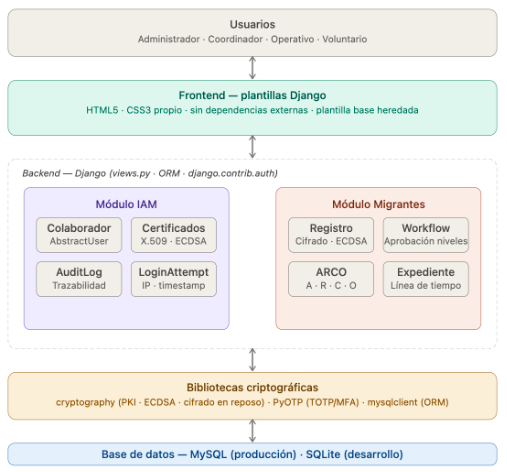
\includegraphics[width=0.9\textwidth]{arquitectura.png}
\captionof{figure}{Diagrama de arquitectura del sistema de gestión de identidades y registro de migrantes de Casa Monarca. Generado con Claude (Anthropic, 2026).}
\label{fig:arquitectura}
\end{center}

\section{Backend}

\subsection{Módulo IAM}

El módulo de gestión de colaboradores tiene 4 modelos:

\begin{itemize}
    \item \textbf{Colaborador:} basado en \texttt{AbstractUser}. Se le agregaron campos específicos de Casa Monarca: área, nivel de acceso, rol, puesto e indicadores de estado (\texttt{is\_revoked}, \texttt{is\_deleted}).
    \item \textbf{UserCertificate:} guarda el certificado X.509 de cada colaborador: emisor, fecha de vencimiento, estado y huella digital.
    \item \textbf{AuditLog:} registra cada acción del sistema con actor, objeto afectado y marca temporal.
    \item \textbf{LoginAttempt:} registra cada intento de inicio de sesión, exitoso o no, con la dirección IP de origen.
\end{itemize}

\textbf{Áreas reconocidas:} Humanitaria, Psicosocial, Legal, Comunicación, Almacén, Tecnologías de la Información.

\textbf{Ciclo de vida de un colaborador:} alta temporal (contraseña temporal) → onboarding → aprobación firmada por el administrador → emisión del certificado (solo Nivel 1 y 2) → baja o revocación. En caso de cinco intentos fallidos de inicio de sesión en 15 minutos, la cuenta queda bloqueada temporalmente.

\subsection{Módulo de Registro de Migrantes}

El módulo de registro tiene 12 modelos:

\begin{itemize}
    \item \textbf{MigrantRegistration:} expediente del migrante. Los campos sensibles (nombre, apellidos, fecha de nacimiento, teléfono, país de origen) se almacenan cifrados con AES-256.
    \item \textbf{MigrantRegistrationSignature:} firma ECDSA del expediente. Relación uno a uno con \texttt{MigrantRegistration}. Guarda los componentes $(r, s)$ de la firma.
    \item \textbf{ActionSignature:} firma para cualquier acción de la plataforma.
    \item \textbf{BatchSignSession:} sesión de firma masiva. Evita solicitar credenciales repetidamente manteniendo la trazabilidad.
    \item \textbf{WorkflowRequest:} solicitud de creación, edición o eliminación por parte de los niveles 3 y 4.
    \item \textbf{ApprovalStep:} decisión de un aprobador sobre un \texttt{WorkflowRequest}.
    \item \textbf{ArcoRequest:} solicitud formal de derechos ARCO.
    \item \textbf{ArcoTicket:} ticket de coordinación del flujo de autorización de una solicitud ARCO.
    \item \textbf{Ticket:} ticket de seguimiento creado automáticamente para cualquier evento.
    \item \textbf{Notification:} notificaciones internas del sistema.
    \item \textbf{RegistrationEvent:} bitácora por expediente.
    \item \textbf{SignedFlowLog:} registro inmutable de acciones irreversibles firmadas con certificado X.509. Es el único modelo del sistema que no permite edición ni eliminación.
\end{itemize}

\textbf{Firma digital de registros:} al crear o editar un expediente, el sistema serializa todos los campos, calcula su resumen SHA-256 y lo firma con ECDSA usando la clave privada del colaborador activo. La firma queda vinculada al expediente en \texttt{MigrantRegistrationSignature}.

\textbf{Eliminación lógica:} cuando un administrador elimina un registro, el sistema activa el campo \texttt{is\_deleted} y registra quién realizó la acción y cuándo. El registro deja de aparecer en el listado activo pero el administrador conserva acceso.

\subsection{Flujo de aprobación (Workflow)}

El sistema implementa un flujo de estados para proteger los movimientos esenciales: \textit{Enviado} → \textit{En revisión} → \textit{Escalado} → \textit{Aprobado} → \textit{Firmado digitalmente} → \textit{Ejecutado} (o \textit{Rechazado} en cualquier punto). Los niveles 1 y 2 pueden ejecutar acciones directamente; los niveles 3 y 4 solo pueden enviar solicitudes que deben ser aprobadas por el coordinador o administrador. La firma de ejecución requiere contraseña, \texttt{.cert} y \texttt{.key} del aprobador.

\subsection{Derechos ARCO}

El sistema implementa los cuatro derechos ARCO conforme a la LFPDPPP \citeref{camara2010}{Cámara de Diputados, 2010}:

\begin{itemize}
    \item \textbf{Acceso:} el beneficiario conoce los datos almacenados (ejecuta Coordinador o Admin).
    \item \textbf{Rectificación:} corrección de datos inexactos, con evidencia adjunta en PDF (ejecuta Coordinador o Admin).
    \item \textbf{Cancelación:} eliminación definitiva de los datos del sistema (solo Admin).
    \item \textbf{Oposición:} el beneficiario se opone a un uso específico de su información (ejecuta Coordinador o Admin).
\end{itemize}

El flujo opera en dos niveles: el coordinador revisa y escala; el administrador aprueba y ejecuta. Cada decisión queda registrada con la firma digital del responsable. Al recibir una solicitud, el sistema calcula automáticamente la fecha límite de respuesta (20 días hábiles desde la recepción, según la LFPDPPP). Cuando se ejecuta una Cancelación, los datos cifrados del migrante son eliminados definitivamente; el registro de auditoría se conserva únicamente para el administrador.

\subsection{Auditoría y trazabilidad}

La trazabilidad opera sobre cuatro elementos simultáneos: el modelo \texttt{AuditLog} captura altas, bajas, aprobaciones de onboarding, emisiones y revocaciones de certificados; \texttt{LoginAttempt} registra cada intento de inicio de sesión con dirección IP; \texttt{RegistrationEvent} une consultas, ediciones, consentimientos, solicitudes ARCO y pasos de aprobación por expediente; y \texttt{ActionSignature} encadena criptográficamente cada firma mediante SHA-256 sobre la firma anterior, formando una cadena de custodia verificable e inalterable.

\section{Frontend}

Para el frontend se utilizaron plantillas de Django con HTML5 y CSS propio, sin dependencias de frameworks externos. Se heredó la plantilla base en todas las pantallas para evitar duplicación de código. Cada pantalla muestra únicamente las acciones disponibles para el nivel del usuario autenticado.

\textbf{Etapa 1 --- Gestión de colaboradores:}

\begin{itemize}
    \item Login (con carga de \texttt{.cert}/\texttt{.key} para Niveles 1 y 2)
    \begin{center}
        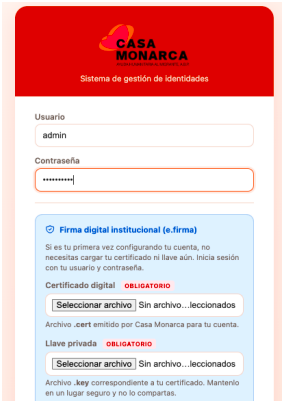
\includegraphics[width=0.85\textwidth]{login.png}
        \captionof{figure}{Pantalla de login con campos de usuario, contraseña y carga de \texttt{.cert}/\texttt{.key} (Niveles 1 y 2) (elaboración propia).}
        \label{fig:login}
    \end{center}
    \item Dashboard de colaboradores
    \begin{center}
        
\includegraphics[width=0.85\textwidth]{dashboard.png}
        \captionof{figure}{Dashboard de colaboradores con tarjetas de estadísticas (elaboración propia).}
        \label{fig:dashboard}
    \end{center}
    \item Onboarding
    \begin{center}
        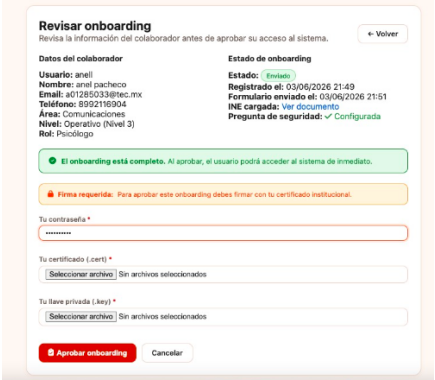
\includegraphics[width=0.85\textwidth]{onboarding.png}
        \captionof{figure}{Formulario de onboarding de nuevos colaboradores (elaboración propia).}
        \label{fig:onboarding}
    \end{center}
    \item Detalle de colaborador
    \begin{center}
        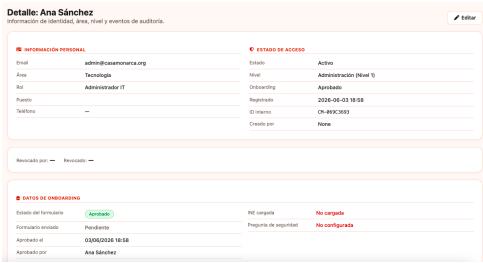
\includegraphics[width=0.85\textwidth]{detalle.png}
        \captionof{figure}{Vista de detalle de un colaborador con historial de acciones (elaboración propia).}
        \label{fig:detalle}
    \end{center}
    \item Auditoría IAM
    \begin{center}
        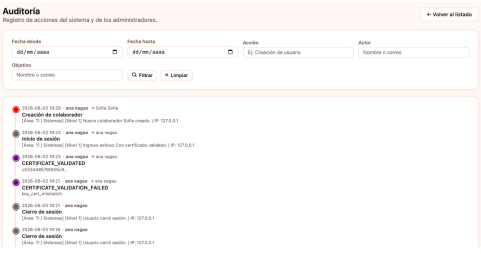
\includegraphics[width=0.85\textwidth]{auditoria.png}
        \captionof{figure}{Módulo de auditoría IAM con filtros por fecha, acción y actor (elaboración propia).}
        \label{fig:auditoria}
    \end{center}
    \item Gestión de certificados
    \begin{center}
        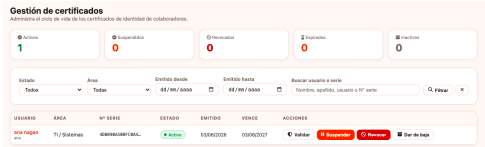
\includegraphics[width=0.85\textwidth]{gestion.png}
        \captionof{figure}{Módulo de gestión de certificados con resumen por estado (elaboración propia).}
        \label{fig:gestion}
    \end{center}
\end{itemize}

\textbf{Etapa 2 --- Registro de migrantes:}

\begin{itemize}
    \item Formulario de nuevo registro
    \begin{center}
        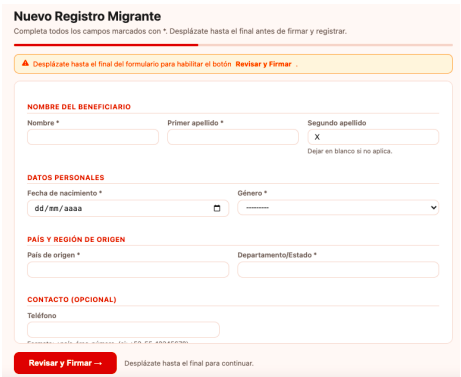
\includegraphics[width=0.85\textwidth]{nuevo.png}
        \captionof{figure}{Formulario de nuevo registro de migrante (elaboración propia).}
        \label{fig:nuevo}
    \end{center}
    \item Revisión y confirmación con firma
    \begin{center}
        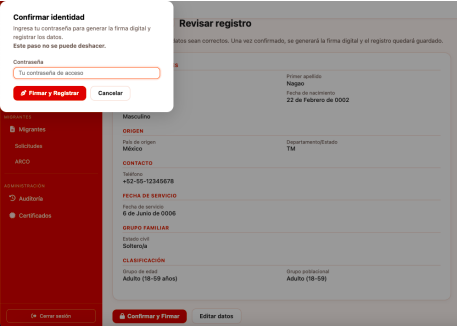
\includegraphics[width=0.85\textwidth]{firma.png}
        \captionof{figure}{Pantalla de revisión y confirmación con solicitud de contraseña para firmar (elaboración propia).}
        \label{fig:firma}
    \end{center}
    \item Listado de registros
    \begin{center}
        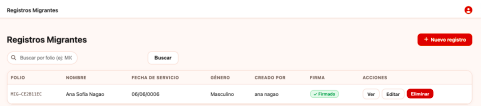
\includegraphics[width=0.85\textwidth]{listado.png}
        \captionof{figure}{Listado de registros de migrantes con buscador por identificador interno (elaboración propia).}
        \label{fig:listado}
    \end{center}
    \item Detalle con firma ECDSA
    \begin{center}
        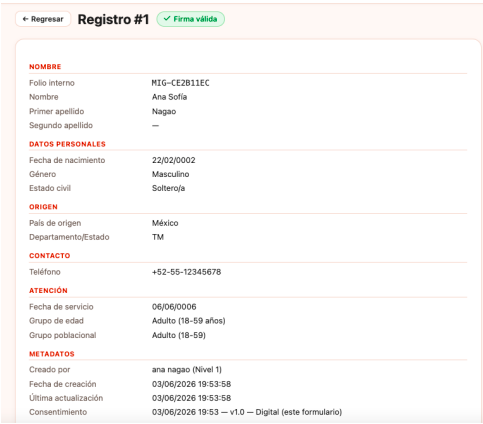
\includegraphics[width=0.85\textwidth]{ECDSA.png}
        \captionof{figure}{Detalle de registro con bloque de firma ECDSA verificada (elaboración propia).}
        \label{fig:ECDSA}
    \end{center}
    \item Expediente completo
    \begin{center}
        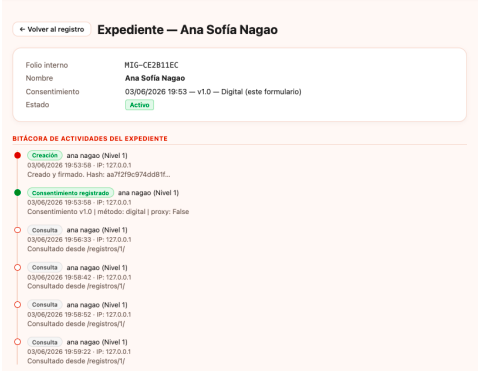
\includegraphics[width=0.85\textwidth]{Expediente.png}
        \captionof{figure}{Expediente completo con línea de tiempo de eventos del registro (elaboración propia).}
        \label{fig:Expediente}
    \end{center}
\end{itemize}

\textbf{Workflow y ARCO:}

\begin{itemize}
    \item Listado de solicitudes
    \begin{center}
        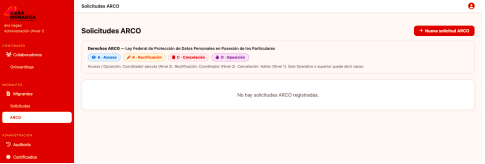
\includegraphics[width=0.85\textwidth]{listsolicitudes.png}
        \captionof{figure}{Listado de solicitudes de cambio con estados del flujo de aprobación (elaboración propia).}
        \label{fig:listsolicitudes}
    \end{center}
    \item Decisión con firma obligatoria
    \begin{center}
        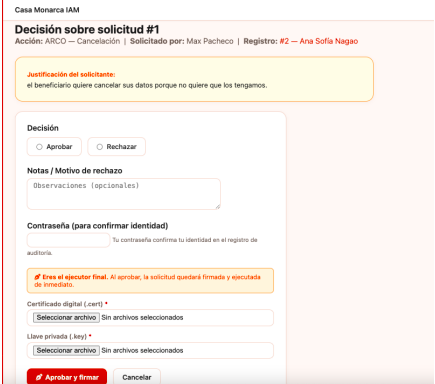
\includegraphics[width=0.85\textwidth]{obligatoria.png}
        \captionof{figure}{Pantalla de decisión sobre solicitud con firma digital obligatoria (elaboración propia).}
        \label{fig:obligatoria}
    \end{center}
    \item Formulario ARCO
    \begin{center}
        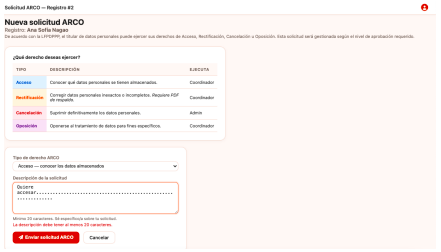
\includegraphics[width=0.85\textwidth]{ARCO.png}
        \captionof{figure}{Formulario de nueva solicitud de derechos ARCO (elaboración propia).}
        \label{fig:ARCO}
    \end{center}
    \item Detalle de solicitud ARCO
    \begin{center}
        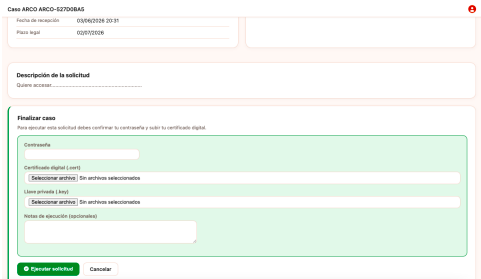
\includegraphics[width=0.85\textwidth]{DETARCO.png}
        \captionof{figure}{Detalle de caso ARCO con flujo de aprobación vinculado y plazo legal calculado (elaboración propia).}
        \label{fig:DETARCO}
    \end{center}
\end{itemize}

\textbf{Perfil:}

\begin{itemize}
    \item Cambio de contraseña
    \begin{center}
        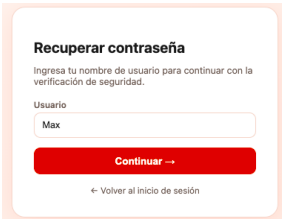
\includegraphics[width=0.85\textwidth]{cambio.png}
        \captionof{figure}{Pantalla de cambio de contraseña (elaboración propia).}
        \label{fig:cambio}
    \end{center}
    \item Configuración de pregunta de seguridad
    \begin{center}
        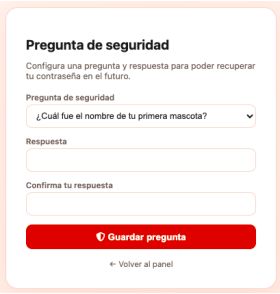
\includegraphics[width=0.85\textwidth]{pregunta.png}
        \captionof{figure}{Configuración de pregunta de seguridad para recuperación de contraseña (elaboración propia).}
        \label{fig:pregunta}
    \end{center}
\end{itemize}

\section{Conexión de componentes}

La comunicación entre los componentes opera en capas. Cuando un usuario realiza una acción desde la interfaz, la petición HTTP llega a los archivos \texttt{views.py} de Django, que verifican la identidad del usuario mediante \texttt{django.contrib.auth}. Para operaciones con datos sensibles, la biblioteca PyCa \textit{cryptography} actúa en dos momentos: al escribir, cifra los campos protegidos del expediente antes de que el ORM los persista; al leer, los descifra. Cuando se crea o edita un registro de migrante, PyCa también calcula el resumen SHA-256 del contenido y genera la firma ECDSA con la clave privada del usuario. Toda comunicación con la base de datos MySQL ocurre exclusivamente a través del ORM de Django mediante \texttt{mysqlclient}; ninguna vista ejecuta SQL directamente, lo que elimina el riesgo de inyección SQL.

% ===========================================================================
% 4. RESULTADOS
% ===========================================================================
\chapter{Resultados}

\section{Backend}

El módulo IAM gestiona el ciclo de vida completo de un colaborador: alta con contraseña temporal, onboarding, aprobación firmada digitalmente, emisión automática del certificado X.509 y baja o revocación. El modelo \texttt{LoginAttempt} permite al administrador identificar comportamientos sospechosos como múltiples intentos fallidos desde una misma IP. El módulo de Registro de Migrantes genera expedientes con cifrado automático de los campos sensibles y firma ECDSA válida al confirmar cada registro.

El flujo de aprobación funciona correctamente para los Niveles 3 y 4: las solicitudes son enrutadas al coordinador o administrador según el tipo de acción; cada aprobación queda respaldada por la firma digital del responsable. Los derechos ARCO están implementados en sus cuatro tipos con flujo de dos niveles. La auditoría cubre la totalidad de los eventos del sistema: acciones IAM, certificados, expedientes, solicitudes ARCO y pasos de aprobación.

\section{Frontend}

Cada pantalla refleja el nivel de acceso del usuario autenticado. La pantalla de login solicita a los colaboradores de Nivel 1 y 2 adjuntar obligatoriamente su certificado digital y su llave privada, mientras que los Niveles 3 y 4 acceden con usuario y contraseña únicamente. Tras cinco intentos fallidos en 15 minutos, la cuenta queda bloqueada temporalmente. El formulario de registro incluye los campos requeridos por Casa Monarca, la captura del consentimiento y la pantalla de revisión previa a la firma.

\section{Solución completa}

El sistema cumple de forma integral con los objetivos del reto. Gestiona el ciclo de vida de un colaborador desde el alta hasta la revocación; registra expedientes de migrantes con datos cifrados y firma ECDSA verificable; aplica control de acceso por niveles; y permite ejercer los derechos ARCO en los plazos legales, generando en todo momento una cadena criptográficamente verificable de quién autorizó cada acción y cuándo.

% ---------------------------------------------------------------------------
\section{Casos de uso y tabla de validaciones}
% ---------------------------------------------------------------------------

Para validar el correcto funcionamiento del sistema se ejecutaron 23 casos de prueba distribuidos en dos módulos: IAM (Inicio de Sesión) y Registro de Migrantes (CRUD). La Tabla~\ref{tab:validaciones_resumen} presenta los casos más representativos de cada funcionalidad crítica; la cobertura completa se documenta en el Anexo~\ref{anx:casos_prueba}.

\textit{Nota:} No se incluyen capturas de todos los casos para mantener la proporción texto/imagen del documento. Las evidencias completas están disponibles en la carpeta \texttt{Casos de Prueba/} del repositorio y en los archivos adjuntos de casos de prueba.

\begin{longtable}{c p{2.0cm} p{3.2cm} p{3.2cm} c}
\caption{Casos de uso representativos y resultados de validación (elaboración propia).}
\label{tab:validaciones_resumen}\\
\toprule
\textbf{\#} & \textbf{Módulo} & \textbf{Caso de uso} & \textbf{Resultado esperado} & \textbf{Estado}\\
\midrule
\endfirsthead
\toprule
\textbf{\#} & \textbf{Módulo} & \textbf{Caso de uso} & \textbf{Resultado esperado} & \textbf{Estado}\\
\midrule
\endhead
\bottomrule
\endfoot
CP-01 & IAM --- Login & Acceso con credenciales válidas & Redirige al dashboard; crea registro en \texttt{AuditLog} & \cmark \\[4pt]
CP-02 & IAM --- Login & Contraseña incorrecta & Mensaje \textit{``Usuario o contraseña incorrectos''}; registra intento fallido & \cmark \\[4pt]
CP-04 & IAM --- Login & Cuenta revocada (\texttt{is\_revoked=True}) & Mensaje \textit{``Cuenta inactiva o revocada. Contacta al administrador.''} & \cmark \\[4pt]
CP-07 & IAM --- Login & Onboarding pendiente & Redirección a \texttt{/onboarding/} con mensaje informativo & \cmark \\[4pt]
CP-08 & IAM --- Login & Aprobado, certificado no descargado & Redirección a descarga de credenciales & \cmark \\[4pt]
REG-01 & Registros --- Create & Registro exitoso & Guardado con firma ECDSA y aparece en lista & \cmark \\[4pt]
REG-02 & Registros --- Create & Sin aceptar aviso de privacidad & Error: \textit{``Debes aceptar el Aviso de Privacidad''} & \cmark \\[4pt]
REG-04 & Registros --- Create & Menores $>$ tamaño del grupo & Error: \textit{``Los menores no pueden superar el tamaño del grupo''} & \cmark \\[4pt]
REG-06 & Registros --- Read & Admin ve todos los registros & Lista completa visible con acciones disponibles & \cmark \\[4pt]
REG-07 & Registros --- Read & Operativo ve registros & Lista filtrada según permisos del nivel & \cmark \\[4pt]
REG-09 & Registros --- Update & Edición directa por admin & Registro actualizado; firma ECDSA recalculada & \cmark \\[4pt]
REG-10 & Registros --- Update & Edición por operativo vía workflow & Solicitud queda en estado \textit{Pendiente de aprobación} & \cmark \\[4pt]
REG-11 & Registros --- Update & Aprobación de cambio propuesto & Cambio se aplica al registro tras firma del coordinador & \cmark \\[4pt]
REG-13 & Registros --- Delete & Eliminación lógica por admin & \texttt{is\_deleted=True}; no desaparece de la BD & \cmark \\[4pt]
REG-14 & Registros --- Delete & Búsqueda de registro eliminado & No aparece en la lista activa normal & \cmark \\
\end{longtable}

Todos los casos ejecutados resultaron aprobados. Las evidencias fotográficas de los casos seleccionados se incluyen en el Anexo~\ref{anx:evidencias}.

% ===========================================================================
% 5. CONCLUSIONES Y TRABAJO FUTURO
% ===========================================================================
\chapter{Conclusiones y Trabajo Futuro}

\section{Conclusiones}

A lo largo de las dos etapas del reto se diseñó e implementó un sistema funcional que apoya en la resolución de las necesidades de Casa Monarca. La Etapa 1 consistió en un gestor de identidades con trazabilidad completa mediante un espacio de auditoría. La Etapa 2 añadió un módulo de registro de migrantes que cifra los datos sensibles con AES-256, firma cada expediente con ECDSA sobre SHA-256, gestiona los cambios mediante aprobación por niveles y permite ejercer los cuatro derechos ARCO en los plazos legales. La cadena criptográfica de auditoría garantiza que el historial de acciones sea verificable e inalterable.

Con esta solución, Casa Monarca dispondrá de herramientas para responder solicitudes ARCO dentro del plazo legal y para detectar brechas de seguridad de forma temprana. Las pantallas guían al usuario paso a paso, los mensajes de error son descriptivos y las acciones irreversibles requieren confirmación explícita con credenciales digitales, reduciendo los errores humanos.

\section{Trabajo futuro}

Los siguientes pasos son el despliegue del sistema en el servidor de Casa Monarca y la capacitación del personal. Se propone adicionalmente el desarrollo de un mecanismo de respaldo automático de la base de datos y un sistema de notificaciones por correo ante cualquier cambio irreversible. Cuando los recursos de Casa Monarca lo permitan, se recomienda migrar a una autoridad certificadora de mayor madurez como step-ca, que ofrece gestión automatizada de renovaciones y soporte ante compromisos de seguridad \citeref{smallstep2026}{Smallstep Labs, 2026}.

% ===========================================================================
% REFERENCIAS
% ===========================================================================
\chapter*{Referencias}
\addcontentsline{toc}{chapter}{Referencias}

\begingroup
\small
\setlength{\parindent}{0pt}
\setlength{\parskip}{6pt}
\sloppy

\begin{description}[leftmargin=0pt, labelwidth=0pt, labelsep=0pt, itemindent=0pt, itemsep=8pt]

    \item[\hypertarget{ref:anthropic2026}{}]
    Anthropic. (2026). \textit{Claude} (Claude Sonnet 4.6) [Modelo de lenguaje de gran escala]. Disponible en: \url{https://www.anthropic.com}

    \item[\hypertarget{ref:boeyen2008}{}]
    Boeyen, S., Santesson, S., Polk, T., Housley, R., Farrell, S., \& Cooper, D. (2008). \textit{Internet X.509 Public Key Infrastructure Certificate and Certificate Revocation List (CRL) Profile} (RFC 5280). RFC Editor. \url{https://datatracker.ietf.org/doc/rfc5280/}

    \item[\hypertarget{ref:camara2010}{}]
    Cámara de Diputados del H. Congreso de la Unión. (2010). \textit{Ley Federal de Protección de Datos Personales en Posesión de Particulares}. Diario Oficial de la Federación. \url{https://www.diputados.gob.mx/LeyesBiblio/pdf/LFPDPPP.pdf}

    \item[\hypertarget{ref:django2026}{}]
    Django Software Foundation. (2026). \textit{Django documentation}. \url{https://www.djangoproject.com/}

    \item[\hypertarget{ref:hankerson2004}{}]
    Hankerson, D., Menezes, A., \& Vanstone, S. (2004). \textit{Guide to Elliptic Curve Cryptography}. Springer. \url{https://doi.org/10.1007/b97644}

    \item[\hypertarget{ref:inegi2020}{}]
    INEGI. (2020). \textit{Tabulados interactivos: Migración}. \url{https://www.inegi.org.mx/app/tabulados/interactivos/?pxq=Migracion_Migracion_01_426da5e7-766a-42a9-baef-5768cde4fca9}

    \item[\hypertarget{ref:johnson2001}{}]
    Johnson, D., Menezes, A., \& Vanstone, S. (2001). The Elliptic Curve Digital Signature Algorithm (ECDSA). \textit{International Journal of Information Security}, \textit{1}(1), 36--63. \url{https://doi.org/10.1007/s102070100002}

    \item[\hypertarget{ref:katz2014}{}]
    Katz, J., \& Lindell, Y. (2014). \textit{Introduction to Modern Cryptography} (2.ª ed.). CRC Press.

    \item[\hypertarget{ref:keycloak2026}{}]
    Keycloak Project. (2026). \textit{Keycloak documentation}. \url{https://www.keycloak.org/}

    \item[\hypertarget{ref:nakamoto2008}{}]
    Nakamoto, S. (2008). \textit{Bitcoin: A Peer-to-Peer Electronic Cash System}. Disponible en: \url{https://bitcoin.org/bitcoin.pdf}

    \item[\hypertarget{ref:nist2001aes}{}]
    National Institute of Standards and Technology. (2001). \textit{FIPS 197: Advanced Encryption Standard (AES)}. NIST. \url{https://nvlpubs.nist.gov/nistpubs/FIPS/NIST.FIPS.197-upd1.pdf}

    \item[\hypertarget{ref:nist2015sha}{}]
    National Institute of Standards and Technology. (2015). \textit{FIPS 180-4: Secure Hash Standard (SHS)}. NIST. \url{https://nvlpubs.nist.gov/nistpubs/FIPS/NIST.FIPS.180-4.pdf}

    \item[\hypertarget{ref:nist2023}{}]
    National Institute of Standards and Technology. (2023). \textit{FIPS 186-5: Digital Signature Standard (DSS)}. NIST. \url{https://nvlpubs.nist.gov/nistpubs/FIPS/NIST.FIPS.186-5.pdf}

    \item[\hypertarget{ref:pyca2024}{}]
    Python Cryptographic Authority. (2024). \textit{cryptography 42.0 documentation}. \url{https://cryptography.io/en/latest/}

    \item[\hypertarget{ref:smallstep2026}{}]
    Smallstep Labs. (2026). \textit{step-ca documentation}. \url{https://smallstep.com/docs/step-ca/}

    \item[\hypertarget{ref:zamora2018}{}]
    Zamora G., J. (2018). \textit{Migración sudamericana en México} [Tesis]. El Colegio de la Frontera Norte. \url{https://posgrado.colef.mx/tesis/uec2017329/}

\end{description}
\endgroup

% ===========================================================================
% ANEXOS
% ===========================================================================
\appendix

\chapter{Tabla completa de casos de prueba}
\label{anx:casos_prueba}

La Tabla~\ref{tab:cp_completo} documenta los 23 casos de prueba ejecutados sobre los módulos IAM (Inicio de Sesión) y Registro de Migrantes (CRUD completo).

\begin{longtable}{c p{1.8cm} p{2.6cm} p{2.0cm} p{2.6cm} c}
\caption{Tabla completa de casos de prueba y validaciones (elaboración propia).}
\label{tab:cp_completo}\\
\toprule
\textbf{\#} & \textbf{Módulo} & \textbf{Caso} & \textbf{Precondición / Entrada} & \textbf{Resultado esperado} & \textbf{Estado}\\
\midrule
\endfirsthead
\toprule
\textbf{\#} & \textbf{Módulo} & \textbf{Caso} & \textbf{Precondición / Entrada} & \textbf{Resultado esperado} & \textbf{Estado}\\
\midrule
\endhead
\bottomrule
\endfoot
% ── IAM: Inicio de Sesión ──────────────────────────────────────────────────
CP-01 & IAM --- Login & Credenciales válidas (sin cert) & Usuario y contraseña válidos & Redirige al dashboard; crea registro en \texttt{AuditLog} & \cmark \\[4pt]
CP-02 & IAM --- Login & Contraseña incorrecta & Usuario válido, contraseña errónea & \textit{``Usuario o contraseña incorrectos''}; intento fallido registrado & \cmark \\[4pt]
CP-03 & IAM --- Login & Usuario inexistente & Usuario que no existe & \textit{``Usuario o contraseña incorrectos''} & \cmark \\[4pt]
CP-04 & IAM --- Login & Cuenta revocada & \texttt{is\_revoked=True} & \textit{``Cuenta inactiva o revocada. Contacta al administrador.''} & \cmark \\[4pt]
CP-05 & IAM --- Login & Cuenta eliminada & \texttt{is\_deleted=True} & \textit{``Cuenta inactiva o revocada. Contacta al administrador.''} & \cmark \\[4pt]
CP-06 & IAM --- Login & Cuenta inactiva & \texttt{is\_active=False} & \textit{``Cuenta inactiva o revocada. Contacta al administrador.''} & \cmark \\[4pt]
CP-07 & IAM --- Login & Onboarding pendiente & \texttt{onboarding\_status='pending'} & Redirige a \texttt{/onboarding/} con mensaje informativo & \cmark \\[4pt]
CP-08 & IAM --- Login & Aprobado, sin cert descargado & \texttt{onboarding\_status='approved'}, \texttt{certificate\_delivered\_at=None} & Redirige a pantalla de descarga de credenciales & \cmark \\[4pt]
CP-09 & IAM --- Login & MFA habilitado, código correcto & OTP válido por TOTP & Acceso concedido; \texttt{AuditLog} indica ``con MFA'' & \cmark \\[4pt]
% ── Registros: Create ─────────────────────────────────────────────────────
REG-01 & Registros --- Create & Registro exitoso & Todos los campos obligatorios completos; aviso de privacidad aceptado & Registro guardado con firma ECDSA; aparece en lista & \cmark \\[4pt]
REG-02 & Registros --- Create & Sin aceptar privacidad & Aviso de privacidad sin marcar & Error: \textit{``Debes aceptar el Aviso de Privacidad''} & \cmark \\[4pt]
REG-03 & Registros --- Create & Sin tipo de asistencia & Ningún tipo de asistencia seleccionado & Error: \textit{``Selecciona al menos un tipo''} & \cmark \\[4pt]
REG-04 & Registros --- Create & Menores $>$ tamaño del grupo & 3 menores, grupo de tamaño 2 & Error: \textit{``Los menores no pueden superar el tamaño del grupo''} & \cmark \\[4pt]
REG-05 & Registros --- Create & Viaja solo con grupo $>$ 1 & \textit{Viaja solo} marcado; grupo $=$ 2 & Error de validación de consistencia & \cmark \\[4pt]
% ── Registros: Read ───────────────────────────────────────────────────────
REG-06 & Registros --- Read & Admin ve todos & Sesión activa como administrador & Lista completa de registros activos visible & \cmark \\[4pt]
REG-07 & Registros --- Read & Operativo ve registros & Sesión activa como operativo & Lista de registros activos accesible & \cmark \\[4pt]
REG-08 & Registros --- Read & Ver detalle de un migrante & Clic sobre un registro activo & Todos los campos del expediente visibles & \cmark \\[4pt]
% ── Registros: Update ─────────────────────────────────────────────────────
REG-09 & Registros --- Update & Edición directa por admin & Admin modifica cualquier campo & Registro actualizado; firma ECDSA recalculada automáticamente & \cmark \\[4pt]
REG-10 & Registros --- Update & Edición por operativo (workflow) & Operativo propone cambio vía workflow & Solicitud en estado \textit{Pendiente de aprobación} & \cmark \\[4pt]
REG-11 & Registros --- Update & Aprobar cambio propuesto & Coordinador aprueba con contraseña & Cambio aplicado al registro & \cmark \\[4pt]
REG-12 & Registros --- Update & Rechazar cambio propuesto & Coordinador rechaza con nota & Registro sin cambios; solicitud en estado \textit{Rechazada} & \cmark \\[4pt]
% ── Registros: Delete ─────────────────────────────────────────────────────
REG-13 & Registros --- Delete & Eliminación lógica (admin) & Admin elimina un registro activo & \texttt{is\_deleted=True} en BD; no desaparece del almacenamiento & \cmark \\[4pt]
REG-14 & Registros --- Delete & Eliminado no aparece en lista & Búsqueda del registro eliminado en lista normal & No aparece en la lista activa & \cmark \\
\end{longtable}

\chapter{Evidencias seleccionadas}
\label{anx:evidencias}

Las siguientes figuras son evidencias representativas de los módulos validados. Las evidencias de todos los casos están disponibles en la carpeta \texttt{Casos de Prueba/} del repositorio.

\begin{figure}[H]
\centering
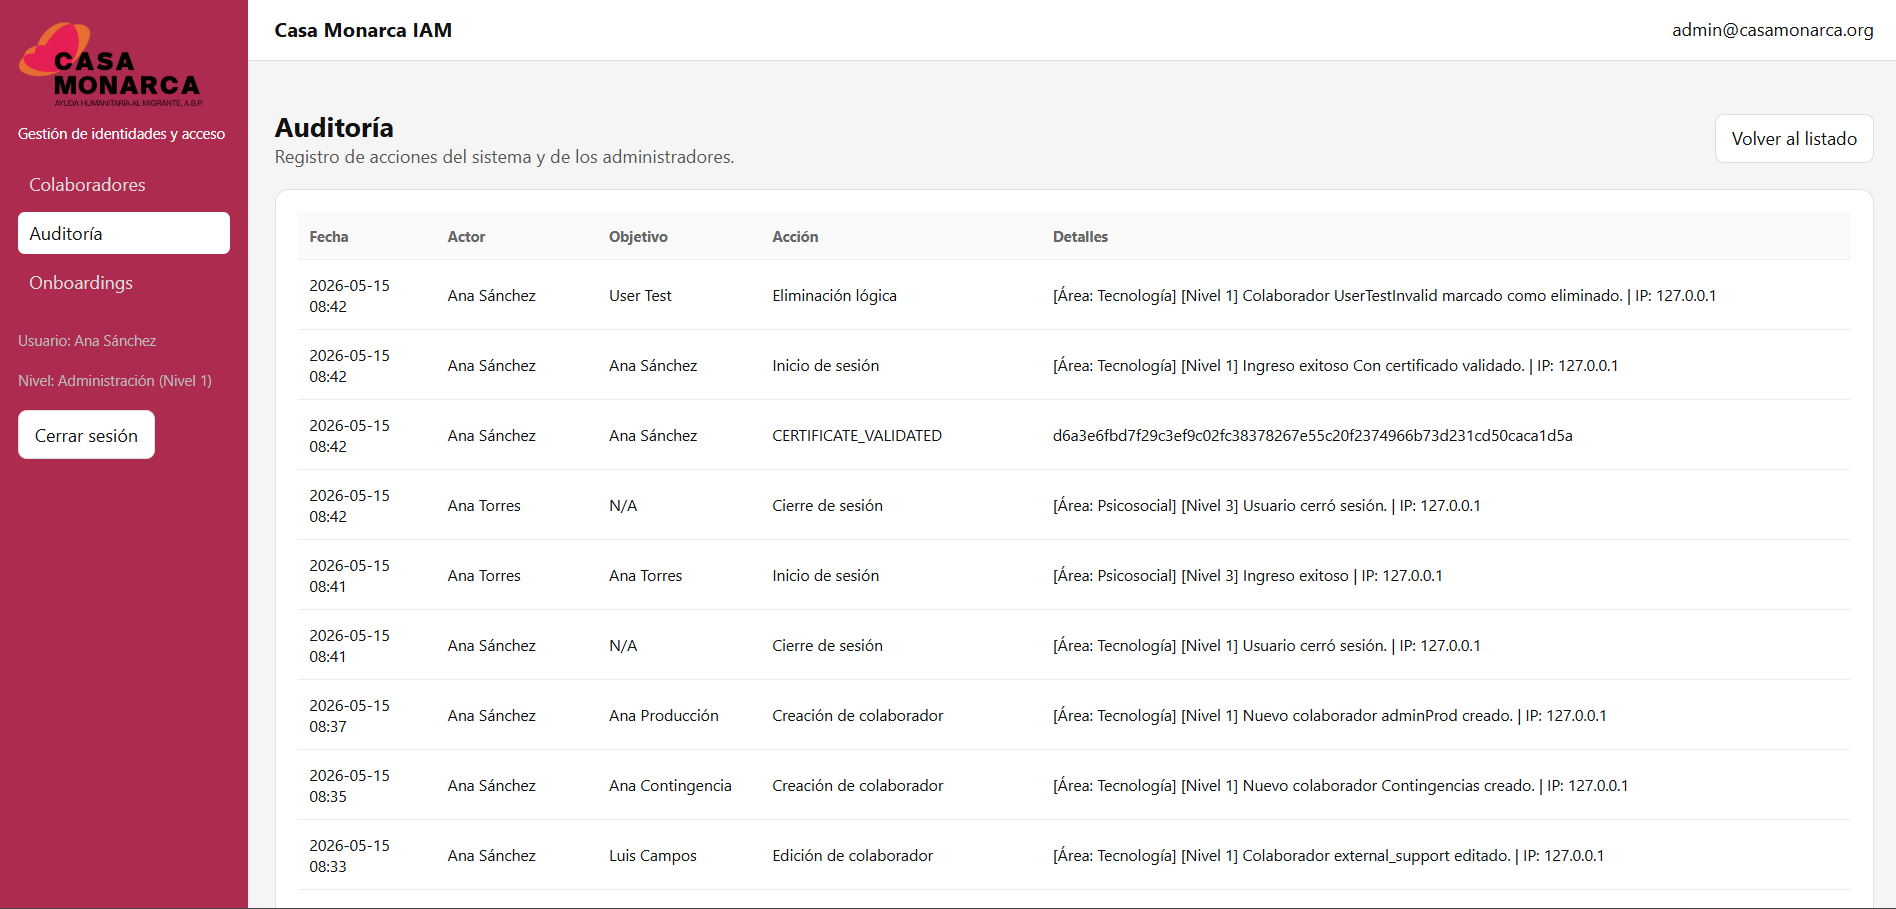
\includegraphics[width=0.85\textwidth]{61/Resultado.png}
\caption{CP-Evidencia --- Vista de registros en la lista (elaboración propia).}
\label{fig:ev61}
\end{figure}

\begin{figure}[H]
\centering

\includegraphics[width=0.85\textwidth]{63/Resultado.png}
\caption{CP-Evidencia --- Detalle de expediente de migrante con datos completos (elaboración propia).}
\label{fig:ev63}
\end{figure}

\begin{figure}[H]
\centering

\includegraphics[width=0.85\textwidth]{65/Resultado.png}
\caption{CP-Evidencia --- Solicitud de cambio en estado de aprobación pendiente (workflow) (elaboración propia).}
\label{fig:ev65}
\end{figure}

\begin{figure}[H]
\centering

\includegraphics[width=0.85\textwidth]{68/Resultado.png}
\caption{CP-Evidencia --- Resultado de aprobación y ejecución de solicitud workflow (elaboración propia).}
\label{fig:ev68}
\end{figure}

\begin{figure}[H]
\centering

\includegraphics[width=0.85\textwidth]{69/Resultado.png}
\caption{CP-Evidencia --- Listado de registros activos tras eliminación lógica de un expediente (elaboración propia).}
\label{fig:ev69}
\end{figure}

\end{document}
